\begin{figure}[t]
    \centering
    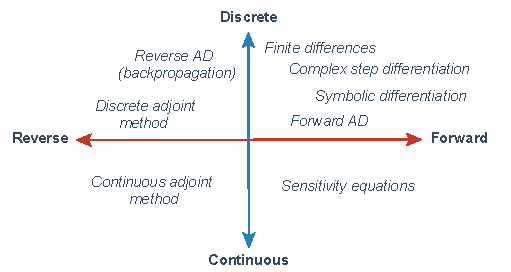
\includegraphics[width=0.80\textwidth]{figures/scheme-methods.pdf}
    \caption{Schematic representation of the different methods available for differentiation involving differential equation solutions. These can be classified depending if they find the gradient by solving a new system of differential equations (\textit{continuous}) or if instead they manipulate unit algebraic operations (\textit{discrete}). Additionally, these methods can be categorized depending if sensitivities are propagated from input to output (forward) or from output to input (reverse).}
    \label{fig:scheme-all-methods}
\end{figure}

There is a large family of methods for computing gradients of functions based on solutions of DEs. 
Depending on the number of parameters and the characteristics of the DE (e.g., level of stiffness), they have different mathematical, numerical, and computational advantages.
These methods can be roughly classified as follows: 
\begin{itemize}
    \item[$\blacktriangleright$] \textit{Continuous} vs \textit{discrete}  methods
    \item[$\blacktriangleright$] \textit{Forward} vs \textit{reverse} methods
\end{itemize}
Figure \ref{fig:scheme-all-methods} displays a classification of some methods under this two-fold division. 

The \textit{continuous} vs \textit{discrete} distinction is one of mathematical and numerical nature. 
When solving for the gradient of a function of the solution of a differential equation, one needs to derive both a mathematical expression for the gradient (the differentiation step) and solve the differential equations using a numerical solver (the discretization step) \cite{bradley2013pde, Onken_Ruthotto_2020, FATODE2014, Sirkes_Tziperman_1997}. 
Depending on the order of these two operations, we refer to discrete methods (discretize-then-differentiate) or continuous methods (differentiate-then-discretize). 
In the case of \textit{discrete} methods, gradients are computed based on simple function evaluations of the solutions of the numerical solver (finite differences, complex step differentiation) or by manipulation of atomic operations inside the numerical solver (AD, symbolic differentiation, discrete adjoint method). 
It is worth noting that although both approaches are classified as discrete methods, their numerical properties are quite different.
In the case of \textit{continuous} methods, a new set of DEs is derived that allow the calculation of the desired gradient, namely the sensitivity (forward sensitivity equations) or the adjoint (continuous adjoint method) of the system.   
% We can either discretize the original system of ODEs in order to numerically solve it and then find an strategy to differentiate it; or instead define new equations for the differentiation step and later numerically solver them.
When comparing discrete to continuous methods, we are focusing, beyond computational efficiency, on the mathematical consistency of the method, that is, \textit{is the method estimating the right gradient?}. 
Discrete methods compute the exact derivative of the numerical approximation to the loss function, but they do not necessarily yield to an approximation of the exact derivatives of the objective function \cite{Eberhard_Bischof_1996, Walther_2007}. 
On the other side, continuous methods lead to consistency error calculation of the sensitivity method \cite{Keulen_Haftka_Kim_2005}. 
% Furthermore, it is important to be aware that when using AD or any other technique we are differentiating the algorithm used to compute the numerical solution, not the numerical solution itself, which can lead to wrong results \cite{Eberhard_Bischof_1996}.
% For example, methods such as automatic differentiation may compute the exact derivative of the numerical approximation of a loss function and yet not give a good approximation of the exact derivative of the loss \cite{Walther_2007}.
% However, one has to keep in mind that AD computes the exact derivative of an approximation of the objective and may not yield an approximation to the exact derivatives of the objective (Section \ref{section:forwardAD-sensitivity}).

The distinction between \textit{forward} and \textit{reverse} regards whether sensitivities are computed for intermediate variables with respect to the input variable or parameter to differentiate (forward) or, on the contrary, we compute the sensitivity of the output variable with respect to each intermediate variable by defining a new adjoint variable (reverse). 
Mathematically speaking, this distinction translates to the fact that forward methods compute directional derivatives by mapping sequential mappings between tangent spaces, while reverse methods apply sequential mappings between co-tangent spaces from the direction of the output variable to the input variable (Section \ref{sec:vjp-jvp}).   
In all forward methods the DE is solved sequentially and simultaneously with the directional derivative during the forward pass of the numerical solver. 
On the contrary, reverse methods compute the gradient by solving a new problem that moves in the opposite direction as the original numerical solver.
In DE-based models, intermediate variables correspond to intermediate solutions of the DE.
In the case of ODEs and time-dependant PDEs, most numerical methods solve the DE by progressively moving forward in time, meaning that reverse methods solve for the gradient moving backwards in time. 
In other words, forward methods compute directional derivatives as they simultaneously solve the original DE, while reverse methods compute adjoints as they solve the problem from output to input.
% \todo[inline]{That doesn't sound right, see Griewank, section 3: the forward model computes directional derivatives, not gradients (tangent mode), the reverse mode computes gradients (adjoint mode). I.e., forward mode maps between tangent spaces, reverse mode maps between cotangent spaces. The text can be corrected if you replace "gradient" more generically by "derivative" (but it then misses the point).}

As discussed in the following sections, forward methods are very efficient for problems with a small number of parameters we want to differentiate with respect to. 
Conversely, reverse methods, though more efficient for a large number of parameters, incur greater memory costs and computational overhead which need to be overcome using different performance tricks. 
With the exception of finite differences and complex step differentiation, the rest of the forward methods (i.e. forward AD, forward sensitivity equations, symbolic differentiation) compute the full sensitivity of the differential equation, which can be computationally expensive or intractable for large systems. 
Conversely, reverse methods are based on the computation of intermediate variables, known as the adjoint or dual variables, that cleverly avoid the unnecessary calculation of the full sensitivity at expenses of larger memory cost \cite{Givoli_2021}. 

% Ommiting this paragraph for this section 
% One extra distinction between methods is with regards to how computationally entangled the numerical solver and the differentiation machinery are. 
% % With the exception of the discrete adjoint methods, this coincides with discrete-continuous classification. 
% However, the construction of the discrete adjoint is based on the numerical solver, something that does not happen with the other discrete methods. 
% While this might not have big conceptual implications, it is an important consideration when using software that integrates numerical solvers and differentiation, a distinction that will help in the discussion in Section \ref{sec:computational-implementation}.

The rest of this section is organized as follows. 
We first introduce some basic mathematical notions to facilitate the discussion of the DP methods (Section \ref{section:preliminaries}).
We then mathematically formalize each of the methods listed in Figure \ref{fig:scheme-all-methods}.
We finally discuss the mathematical foundations of these methods in \ref{section:compatison-math} with a comparison of some mathematical foundations of these methods. 
% More specificlacy, our goal here is try to enlight the closed resamblance of the methods 